
%(BEGIN_QUESTION)
% Copyright 2006, Tony R. Kuphaldt, released under the Creative Commons Attribution License (v 1.0)
% This means you may do almost anything with this work of mine, so long as you give me proper credit

Graph {\it just the derivative response} a proportional+derivative controller to the following input conditions, assuming a proportional band of 250\% and a derivative constant of 4 minutes.  The controller's action is {\it reverse}, and the algorithm it follows is shown below the graph:

$$\includegraphics[width=15.5cm]{i01548x01.eps}$$

The time scale on the chart is minutes:seconds, and the P+D algorithm is as follows:

$$m = K_p \left( e + \tau_d {de \over dt} \right) + b$$

\noindent
Where,

$m$ = Controller output (manipulated variable)

$K_p$ = Gain

$e$ = Error signal (SP$-$PV)

$\tau_d$ = Derivative time constant

$b$ = Bias

\vskip 10pt

\underbar{file i01548}
%(END_QUESTION)





%(BEGIN_ANSWER)

$$\includegraphics[width=15.5cm]{i01548x02.eps}$$

First, let us understand that a proportional band of 250\% is equivalent to a gain ($K_p$) of 0.4.  Also, we must realize that as a reverse-acting controller, the output will go in the same direction as the SP, but opposite that of the PV.
 
\vskip 10pt

As the SP descends 5\% between 0:15 and 0:45, it creates a de/dt slope of -10\% per minute.  This figure, times $\tau_d$ = 4 and times $K_p$ = 0.4 gives us a derivative term contribution of -16\%.  Thus, the output steps down from 40\% to 24\% during this time.

When the PV descends at the same rate between 0:45 and 1:15, derivative action drives the output up by the same amount (16\%), from 40\% to 56\%.

Between 1:15 and 2:10, there is no change of error between PV and SP, even though ramping takes place between 1:15 and 1:45.  At 2:15, the positive SP step-change causes the output to saturate at 100\% momentarily, then return to 40\%.

From 2:20 to 2:35, the SP slopes downward 5\%, for a de/dt rate of -20\% per minute.  This gives a derivative response of -32\%, stepping the output down from 40\% to 8\%.  At time 2:35 when the SP stops ramping, the derivative action ceases and the output returns to 40\%.

%(END_ANSWER)





%(BEGIN_NOTES)


%INDEX% Control, proportional + derivative: graphing controller response

%(END_NOTES)


